
\documentclass[11pt,a4paper]{report}

\usepackage{fancyhdr}
\usepackage{amssymb}
\usepackage{amsmath}
\usepackage{graphicx}
\usepackage[T1]{fontenc}
\usepackage{hyperref}
\hypersetup{colorlinks=true,linkcolor=cyan, citecolor=green,filecolor=black,urlcolor=blue}
\usepackage{epstopdf}
\usepackage{makeidx}
\usepackage{tocloft}
\usepackage{tikz}
\usetikzlibrary{shapes,shadows,arrows}

\tikzstyle{startstop} = [rectangle, rounded corners, minimum width=2cm, minimum height=1cm,text centered, draw=black, fill=red!30]
\tikzstyle{io} = [trapezium, trapezium left angle=70, trapezium right angle=110, minimum width=3cm, minimum height=1cm, text centered, draw=black, fill=blue!30]
\tikzstyle{process} = [rectangle, minimum width=5cm, minimum height=1cm, text centered, text width=5cm, draw=black, fill=orange!30]
\tikzstyle{decision} = [diamond, minimum width=3cm, minimum height=1cm, text centered, draw=black, fill=green!30]

\renewcommand{\cftchapleader}{\cftdotfill{\cftdotsep}}
\renewcommand{\contentsname}{Cuprins}
\renewcommand{\bibname}{B\lowercase{ibliografie}}
\renewcommand{\chaptername}{Capitol}
\renewcommand{\appendixname}{Anexa}
\renewcommand{\indexname}{I\lowercase{indice}}
\pagestyle{fancy}
\makeindex
\newtheorem{prop}{Propozi\c tie}
\newenvironment{demo}{\paragraph{\textbf{Demonstra\c{t}ie}:}}{\hfill$\square$}
\newcommand{\R}{\mathbb{R}}
\tikzstyle{arrow}=[thick,-,>=stealth]
\begin{document}
	\pagenumbering{roman}
	

\begin{titlepage}
	\begin{center}
		\large
		\textsc{Universitatea ,\hspace{-0.02cm},Alexandru Ioan Cuza'', Ia\c si}\\
		\textsc{Facultatea de Matematic\u{a}}\\[0.3cm]
 		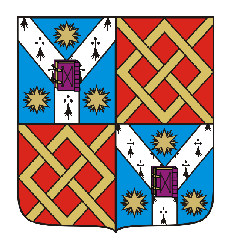
\includegraphics[scale=.4]{stema.eps}
		\vfill
		
		%Titlu
		\Huge
		\textsc{Algoritmi pentru grafuri \c si aplica\c{t}ii}\\[0.8cm]
		\large
		\textbf{Lucrare de licen\c t\u a}
		
		\vfill
		\begin{minipage}[t]{0.49\textwidth}
			\begin{flushleft}
				\large
				\textbf{Conduc\u{a}tor \c{s}tiin\c{t}ific:}\\
				Lect.Dr. Ana-Maria Mo\c{s}neagu
			\end{flushleft}
		\end{minipage}
	    \hfill
	    \begin{minipage}[t]{0.49\textwidth}
	    	\begin{flushright}
	    		\large
	    		\textbf{Student:}\\
	    		Galbini\c t\u a Sebastian
	    	\end{flushright}
    	\end{minipage}
	    
	    \vfill
	    \large
	    \centering
	    Septembrie, 2020\\
	    Ia\c{s}i
	\end{center}
\end{titlepage}

	\tableofcontents
	\thispagestyle{empty}
	\fancyhf{}
	\clearpage
	\pagenumbering{arabic}
	
	\chapter*{Introducere}
	\addcontentsline{toc}{chapter}{Introducere}	
	Multe aplica\c tii computa\c tionale invoc\u a nu numai o pereche de obiecte dar si un set de conexiuni care s\u a lege aceste informatii \^intre ele. Rela\c tia impus\u a de aceste conexiuni a condus la mai multe \^intreb\u ari precum: Exist\u a posibilitatea s\u a ajungi de la un obiect la altul urm\u arind conexiunile? La c\^ ate obiecte pot s\u a ajung pornind de la unul deja prestabilit? Care ar fi cel mai scurt/lung drum parcurs pentru a ajunge la destina\c tia propus\u a? Exist\u a o leg\u atura \^ intre toate tipurile de date? Pentru a ilustra diversitatea aplica\c tiilor ce folosesc propriet\u a\c ti \c si metode, care au ca fundament grafurile, enumer\u am urm\u atoarele exemple: H\u ar\c tile, Hypertexts(documente ce con\c tin referin\c te c\u atre alte pagini web), Circuite, Planific\u ari, Tranzac\c tii, Re\c tea de internet etc.
	
	Pentru a putea r\u aspunde la intreb\u arile de mai sus, vom folosi obiecte abstracte cum ar fi grafurile. Grafurile sunt structuri de date extrem de r\u asp\^ andite \^ in \c stiin\c ta calculatoarelor, iar algoritmii de grafuri sunt esen\c tiali in acest domeniu.
	
	\^ In  capitolul 1 se trateaz\u a problema de a determina toate drumurile de cost minim dintre oricare doua noduri \c si determinarea drumurilor minime de la un nod fixat la toate celelalte, c\^ and fiecare muchie are asociat\u a o lungime.
	
	\^ In capitolul 2 se v-a descrie determinarea unui arbore de acoperire minim\u a al unui graf. Acest arbore este introdus ca fiind  cea mai "ieftin\u a" cale de conectare a tuturor v\^ arfurilor atunci c\^ and fiecare dintre muchie are un cost asociat. Algoritmii de acoperire minim\u a a unui graf sunt exemple concrete de algoritmi greedy.
		
	\^ In final, \^ in capitolul 3 se v-a discuta despre modul de a putea calcula fluxul maxim de material dintr-o rea\c tea(graf orientat) av\^ and in ipoteza ipoteza sursa de material, destina\c tia \c si cantita\c tile de material care pot traversa muchia.
	
	Pentru evaluarea timpului de execu\c tie al unui algoritm pe un graf fixat $G=(V,E)$, de obicei vom m\u asura dimensiunile intr\u arii  in func\c tie a num\u arului de v\^ arfuri $|V|$ \c si a num\u arului de muchii $|E|$ ale grafului. Astfel exist\u a doi parametrii relevan\c ti care descriu dimensiunea intr\u arii.
	\chapter{No\c tiuni introductive}
	    
	
	Vom incepe studiul cu o introducere in acest capitol a c\^ atorva concepte de baza \^ in teoria grafurilor. Se vor stabili c\^ ateva rezultate ca implic\u a aceste concepte. Aceste rezultate, vor servi, \^ in introducerea cititorului la anumite tehnici utilizate frecvent in dovedirea teoremelor \^ in teoria grafurilor.
	
	\section{Graf}
	
    Un \textit{graf} $G=(V,E)$ este o pereche  de mul\c timi astfel \^ inc\^ at $E\subseteq [V]^2$, astfel elementele din $E$ sunt perechi de dou\u a subseturi de elmente ale lui $V$. Pentru a evita ambiguita\c tile nota\c tionale , vom presupune tacit c\u a $V\cap E=\emptyset$. Elementele din mul\c timea $V$ se numesc \textit{v\^ arfuri}(sau \textit{noduri} sau \textit{points}) ale grafului $G$, elementele multimii $E$ se numesc \textit{muchii}(sau \textit{linii}). Modul obi\c snuit de a ilustra u graf este prin desenarea unui punct pentru fiecare v\^ arf \c si unirea celor dou\u a puncte printr-o linie daca cele doua varfuri corespunz\u atoare formeaza o muchie.
	
	
	\begin{figure}[!hbt]
		\centering
		\includegraphics[width=10.2cm]{Figura1.png}
		\caption{Graful pe $V=\{ 1,2,3...7\}$ cu setul de muchii \centering \newline $E=\{ \{1,2\},\{1,5\},\{2,5\},\{3,4\},\{5,7\} \}$ }
		\end{figure}
	
	Se spune c\u a un graf cu setul de noduri $V$ este un graf pe $V$. Setul de noduri al unui graf $G$ este denumit $V(G)$, muchia s-a fiind $E(G)$. Aceste conven\c tii sunt independente de orice alte denumiri ale acestor dou\u a seturi: setul de noduri $W$ a grafului $H=(W,F)$ este tot definit ca fiind $V(H)$, nu ca $W(H)$. Num\u arul de noduri ale unui graf $G$ este \textit{ordinea} sa, scris\u a ca $|G|$; num\u arul sau de muchii este notat cu $||G||$. Graficele  sunt \textit{finite},\textit{infinite} sau \textit{num\u arabile}. Pentru \textit{graful null} $(\emptyset,\emptyset)$ scriem pur \c si simplu $\emptyset$. Un graf de ordin 0 sau 1 se numeste \textit{trivial}.
	
	Un nod $v$ este \textit{incident} cu o muchie $e$ dac\u a $v\in e$; atunci $e$ este o muchie la $v$. O muchie $\{u,v\}$ este de obicei scris\u a sub forma $(u,v)$. Dac\u a $x\in X$ si $y\in Y$ atunci $(x,y)$ este o muchie $X-Y$. Mul\c timea tuturor marginilor $X-Y$ dintr-un set $E$ este notat cu $E(X,Y)$.
	
	Doua noduri ale grafului $G$ sunt \textit{adiacente}, sau \textit{vecine} dac\u a $(x,y)$ formeaz\u a o muchie pe $G$. Dac\u a toate v\^ arfurile lui $G$ sunt perechi adiacente, atunci $G$ este \textit{complet}. Un graf complet de $n$ v\^ arfuri este un $K^n$; $K^3$ se nume\c ste triunghi.
	
	Fie $G=(V,E)$ \c si $G'=(V',E')$ dou\u a grafuri. Numim $G$  \c si  $G'$  \textbf{izomorfe} \c si not\u am $G\simeq G'$ dac\u a exist\u a o bijectie $\varphi :V\rightarrow V'$ cu $(x,y)\in E  \Leftrightarrow \varphi (x) \varphi (y) \in E'$ pentru orice $x,y\in V$.
	
	\begin{figure}[!hbt]
		\centering
		\includegraphics[width=12.2cm]{Figura2.png}
		\caption{Reuniunea, diferen\c ta si intersec\c tia; v\^ arfurile 2,3,4 \centering \newline formeaz\u a un triunghi \^ in $G\cup G'$ dar nu in $G$}
	\end{figure}
	
	
	Stabilim c\u a $G\cup G'=(V\cup V',E\cup E')$ \c si $G\cap G'=(V\cap V',E\cap E')$. Dac\u a $G\cap G'=\emptyset$, atunci $G$ \c si $G'$ sunt \textit{disjuncte}. Dac\u a $V'\subseteq V$ \c si $E'\subseteq E$, atunci $G'$ este un \textit{subgraf} al ui $G$ (\c si $G$ este un \textit{supergraf} pentru $G'$), scris ca $G'\subseteq G$. Mai pu\c tin formal , spunem ca $G$ il con\c tine pe $G'$. 
    
    \section{Reprezentarea unui graf}
   
   
    Exist\u a dou\u a moduri de reprezentare a unui graf $G=(V,E)$: ca o colectie de list\u a de liste de adiacen\c ta\u asau ca o matrice de adiacen\c t\u a. Oricare dintre aceste dou\u a  modalit\u a\c ti de reprezentare se aplic\u a at\^ at grafurilor orientate c\^ at \c si celor neorientate.
    
    \textbf{Reprezentarea prin liste de adicaen\c t\u a} a grafului $G=(V,E)$ const\u a \^ in realizarea unui tablou $AD$ cu |V| liste, o list\u a pentru fiecare v\^ arf din $V$. Pentru fiecare $u\in V$, $AD[u]$ con\c tine toate v\^ arfurile $v$ astfel \^ inc\^ at exist\u a o muchie $(u,v)\in E$. Figura 1.3(b) este o reprezentare prin liste de adiacen\c t\u a a grafului neorientat din Figura 1.3(a). At\^ at pentru grafurile orientate c\^ at \c si pentru cele neorientate, reprezentarea lor prin liste de adiacen\c t\u a au o dimensiunea de memorie de $O(max(V,E))=O(V+E)$.
    
    Listele de adiacen\c t\u a pot fi adaptate \c si pentru realizara unor \textbf{grafuri cu cost} astfel, pentru fiecare muchie a grafulu $G$ i se asociaz\u a o func\c tie numit\u a \textbf{func\c tie de cost} $\varphi :E\to \R $, unde costul $\varphi(u,v)$ al muchiei $(u,v)$ este memorat \^ impreun\u a cu $v$ \^ in $AD[u]$.
    
    \^ In majoriattea cazurilor, liste de adiacen\c t\u a se folosesc atunci c\^ and vrem sa gestion\u am memoria programului c\^ at mai eficient. De exemplu, dac\u a avem un graf \textit{rar} ($|E|$ este mult ma mic dec\^ at $|V|\times |V|$) \c si am folosi reprezentarea grafului cu ajutorul matricilor, atunci majoritatea elementelor din matrice ar r\u am\^ ne nefolosite produc\^ and astfel o risip\u a de memorie.
    	\begin{figure}[!hbt]
    	\centering
    	\includegraphics[width=13.2cm]{Figura4.png}
    	\caption{Dou\u a reprezent\u ari a unui graf neorientat.(\textbf{a}) Graf  neorientat. \centering \newline(\textbf{b}) List\u a de adiacen\c ta pentru $G$.(\textbf{c}) Matricea de adiacen\c t\u a a lui $G$.}
    \end{figure}

    \begin{figure}[!hbt]
	\centering
	\includegraphics[width=13.2cm]{Figura5.png}
	\caption{Dou\u a reprezent\u ari a unui graf orientat.(\textbf{a}) Graf orientat. \centering \newline(\textbf{b}) List\u a de adiacen\c ta pentru $G$.(\textbf{c}) Matricea de adiacen\c t\u a a lui $G$.}
    \end{figure}
    
    
    Pentru \textbf{reprezentarea prin matrice de adiace\c t\u a}, presupune c\u a v\ arfurile sunt numerotate arbitrar. Reprezentarea matricii de adiacen\c t\u a a grafului $G=(V,E)$ const\u a \^ intr-o matrice $A_{|V|\times |V|}=(a_{ij})$ a.\^ i.:
    \begin{equation*}
    a_{ij}=\begin{cases}
    1, (i,j)\in E \medskip \\
    0, (i,j)\notin E
    \end{cases}
    \end{equation*}
    
    Figuriele 1.3(c) \c si 1.4(c) sunt reprezent\u arile matricilor de adiacen\c t\u a a grafurilor 1.3(a), respectiv 1.4(a). Necesarul de memorie este de $\Theta(V^2)$ \c si nu depinde de num\u a rul de muchii a grafului. \^ In plus, c\^ and se face implementarea cu ajutorul matricilor, verificarea dac\u a este o muchie \^ intre cele dou\u a v\^ arfuri dureaz\u a $\Theta(1)$ timpi, \^ in timp ce cu ajutorul listelor de adiacen\c t\u a ar putea avea un ordin de complexitate liniar $\Theta(n)$.
    
    La fel ca \c si la listele de adiacen\c t\u a, pot fi folosite \c si pentru grafuri cu cost. Astfel, fie un graf cu cost $G=(V,E)$ \c si fie func\c tia de cost $\varphi$ de mai sus , costul $\varphi(u,v)$ al unei muchii $(u,v)\in E$ este memorat ca un element din matrice. \^ In cazul \^ in care o muchie nu exist\u a, elementul corespunz\u ator din matrice poate fi $NIL$ sau \^ in majoritatea cazurilor $0$ sau$\infty$.
    
    Un avantaj pentru folosirea matricilor in locul listelor este acela c\u a dac\u a graful este \textit{dens} ($|E|$ este aproxiativ egal cu  $|V|\times |V|$) atunci num\u arul de muchii este aproape de (complet) $n(n-1)/2$ sau de $n^2$, unde $n=|V|$, dac\u a graful este orientat \c s ciclic.
    \section{Gradul unui v\^ arf}
    
   Reprezentarea unui graf $G=(V,E)$ prin liste de adiacen\c t\ a const\u a intr-un tablou 
    
    Fie $G=(V,E)$ un graf nenul. Mul\c timea vecinilor nodurilor  $v$ \^ in $G$ este notat\u a cu $N_G(v)$ sau pe scurt $N(v)$. Mai general, pentru $U\subseteq V$, vecinii din $V\setminus U$ ai nodurilor din $U$ se numesc vecini lui $U$; mul\c timea lor este notata cu $N(U)$.
    
    \textbf{Gradul} $d_G(v)=d(v)$ a unui v\^ arf $v$  este numarul de muchii $|E(v)|$ la $v$. Dac\u a gradul unui nod este $0$ atunci aceste se nume\c ste \textit{nod izolat}. Num\u arul $\delta(G)=min\, \{\,d(v)\, |\, v\in V\, \}$ este \textit{gradul minim}  lui $G$, iar numarul $\Delta(G)=max\, \{\, d(v)\, |\, v\in V\,\}$ este \textit{gradul maxim}  lui $G$. Dac\u a toate nodurile lui $G$ au acela\c si grad $k$, atunci $G$ este \textit{k-regulat}, sau simplu \textit{regulat}. Un graf 3-regulat se numeste \textit{cub}.
    
    Num\u arul
        \begin{equation*}
    d(G)=\frac{1}{|V|} \sum\limits_{v\in V} d(v)
    \end{equation*}
    se nume\c ste \textit{gradul mediu }a lui $G$. Deasemena, este indus\u a de rela\c tia,
    \begin{equation*}
    \delta(G)\le d(G)\le \Delta(G)
    \end{equation*}
    
    
    
    \section{Dumuri si cicluri}
    \textit{Drumul} este un graf nenul $P=(V,E)$ de forma 
    \begin{equation*}
    V=\{v_1,v_2,....,v_k\}\quad E=\{(v_0,v_1),(v_1,v_2),....,(v_{k-1},v_k)\}
    \end{equation*}
    unde toate nodurile $v_i$ sunt distincte. Nodurile $v_0$ \c si $v_j$ sunt \textit{legate} de $P$ si se numesc \textit{capete}; nodurile $v_1,v_2,...,v_{j-1}$ sunt nodurile interioare ale lui $P$. Num\u arul de muchii a unui drum este \textit{lungimea } lui.
    
    Fiind date doua mul\c timi $A,B$ de noduri, spunem ca $P=[\,x_0,x_1,..,x_k\,]$ este un \textit{drum A-B} dac\u a $V(P)\cap A=\{x_0\}$ \c si $V(P)\cap B=\{x_k\}$. Dou\u a sau mai multe drumuri sunt \textit{independente} dac\u a nici unul dintre ele nu con\c tine un nod interior al altuia. De exemplu, dou\u a drumuri $a-b$ sunt independente d.d $a$ \c si $b$ sunt singurele lor noduri comune.
    
    Dac\u a $P=x_0,..x_{k-1}$ este un drum si $k\ge 3$, atunci graful $C=P+(x_{k-1},x_0)$ este un \textit{ciclu}. Ca \c si la drumuri, vom nota ciclul dupa secven\c ta de noduri pe care o are; ciclul de mai sus $C$ poate fi scris  sub forma $C=[\,x_0,...,x_{k-1},x_0\,]$.
    
    \textit{Distan\c ta} dintre do\u a noduri \^ in $G$ $d_G(x,y)$ este lungimea celui mai scurt drum $x-y$ \^ in $G$; dac\u a nu exist\u a un astfel de drum vom nota $d(x,y)=\infty$. Cea mai mare distan\c ta dintre oricare dou\u a noduri \^ in $G$ este \textit{diametrul} lui $G$, notat\u a cu diam $G$.
    
   %% \begin{prop}
    %%	Orice graf $G$ de con\c tine un drum de lungime $\delta(G)$ si un ciclu de lungime m\u acar $\delta(G)+1$(numai pentru $\delta(G)\ge 2$)
     %%\end{prop}
    %%\begin{demo}
    %%	Fie $x_1,...,x_k$ cel mai lung drum al lui $G$, care nu poate fi extins. Orice vecin a lui $x_1$ trebuie s\u a fie pe drum, deoarece %%altfel am putea s\u a o extindem. \^ Intruc\^ at $x_1$ are m\u acar $\delta (G)$ vecini, atunci mul\c timea $\{x_2,x_3,...,x_k\}$ trebuie %%s\u a con\c tin\u a $\delta (G)$ elemente. Prin urmare $k\ge \delta (G)+1$, are lungimea drumului de cel pu\c tin $\delta (G)$.
    %%\end{demo}
    \section{Conexitate}
    
    Un graf nenul $G=(V,E)$ s.n.y \textit{conex} dac\u a pentru orice $u,v\in V \,$,$u\neq v$ exist\u a cel pu\c tin un drum de la $u$ la $v$. Un subgraf maximal conex la $G$  se nume\c ste \textit{component\u a conex\u a} la $G$. Mai general, pentru orice subgraf $S=(V_1,E_1)$ la $G$, $S$ este convex \c si nu exist\u aun alt subgraf la $G$, $S'=(V_2,E_2)$ cu $V_1\subset V_2$ care s\u a fie conex. Un graf care are la baz\u a un singur nod se nume\c ste graf conex.
    
    Pentru grafurile orientate, vom eviden\c tia dou\u a no\c tiuni asociate cu no\c tiunea de conexitate. 
    Un graf orientat se numește \textit{slab conex} dacă înlocuirea tuturor muchiilor orienatte cu muchii ale unu graf neorientat produce un graf conex (neorientat).
    
    Fie $G$ un graf orientat, se spune c\u a nodurile $x$ \c si $y$ sunt \textit{tare conexe} dac\u a exist\u a simultan un drum de la $x$ la $y$, \c si de la $y$ la $x$, unde cele dou\u a va\^ arfuri sunt distincte \^ intre ele.
   
   	
   
    \chapter{Drumuri minime de surs\u a unic\u a}

    
    S\u a presupunem c\u a un ciclist dore\c ste s\u a parcurga drumul de la Ia\c si la Bac\u au acest\u a utiliz\^and o hart\u a rutier\u a a Rom\^ aniei, unde sunt indicate distan\c tele \^ intre fiecare dou\u a intersec\c tii adiacente.
    
    O posibil\u a rezolvare a acestei probleme este aceea de a \^ in\c sirui toate drumurile de la Ia\c si la Bac\u au \c si, pe baza lungimilor acestora, de a alege cel mai scurt drum dintre ele. Este vizibil de observat faptul c\u a num\u arul de variante posibile este un num\u ar foarte mare chiar \c si \^ in cazul \^ in care avem drumuri care nu con\c tin cicluri.
    
    \^ In acest capitol vom demonstra cum poate fi rezolvat\u a problema \^ in mod eficient. \^ Intr-o \textbf{problem\u a de drum minim}, avem \^ in ipotez\u a un graf orientat ponderat $G=(V,E)$, iar func\c tia cost $w:E \longrightarrow \R $ repartizeaz\u a fiec\u arei muchii un cost exprimat intr-un numar real. \textbf{Costul} drumului  $p=\langle \alpha_{0},\alpha_{1},....,\alpha_{k}\rangle$ reprezint\u a suma costurilor corespunz\u atoare muchiilor componente :
    \begin{equation*}
    f(p)=\sum\limits_{i=1}^{k} f(\alpha_{i-1},\alpha_{i})
    \end{equation*}
    
    A\c sadar, \textbf{costul unui drum minim} de la $u$ la $v$ este dat de
  	\begin{equation*}
  		w(u,v)=
  		\begin{cases}
  	    min\left\{f(p):u\leadsto v\right\},&\text{dac\u a exist\u a drum de la $u$ la $v$} \medskip\\
  		\infty,& \text{altfel} \medskip
  		\end{cases}
  		\end{equation*}
  		
  	In cazul exemplului de mai sus, putem modela harta rutier\u a ca un graf: v\^arfurile constitue punctele de intersec\c tie, muchiile reprezint\u a segmentele de drum iar costurile distan\c tele \^ intre intersec\c tii.
  	
  	\section{Reprezentarea drumurilor minime}
  	
  	Find dat un graf $G=(V,R)$, se v-a re\c tine pentru fiecare v\^ arf $v\in V$ un \textbf{predecesor} $\omega[v]$ care este fie un v\^ arf, fie NULL. Pentru determinarea drumurilor minime, algoritmii prezenta\c ti in acest capitol determin\u a $\omega$ a\c sa \^ inc\^ at pentru orice v\^ arf $v$, lan\c tul de predecesori care porne\c ste de la $v$ s\u a coincid\u a unei tranvers\u ari in ordinea invers\u a unui drum de valoare minim\u a de la $s$ la $v$.
  	
  	Pe durata execu\c tiei a unui algoritm pentru determinarea a unui drum minim, valorile lui $\omega$ nu arat\u a in mod necesar drumurile minime. Astfel, vom considera \textbf{subgraful predecesor} $G_{\omega}=(V_{\omega},E_{\omega})$ indus\u a \^ in valorile lui $\omega$, unde $V_{\omega}$ reprezint\u a mul\c timea v\^ arfurilor din $G$ cu proprietatea c\u a au predecesor diferit de NULL, reunit\u a cu mul\c timea constituit\u a din v\^arful $s$ :
  	
  	\vspace{0.3cm}	
  	$\centering V_{\omega}=\left\{v\in V :\omega[v]\ne NULL\right\}\cup \left\{s\right\}$
  	\vspace{0.3cm}
  		
  	Mul\c timea de muchii $E_{\omega}$ este mul\c timea de muchii impus\u a de valorile lui $\omega$ pentru v\^ arfurile din $V_{\omega}$ :
  	
  	\vspace{0.3cm}
  	$\centering E_{\omega}=\left\{(\omega [v],v)\in E : v\in V_{\omega}\setminus \left\{s\right\}\right\}$
  	\vspace{0.3cm}
  	
  	Fie $G=(V,E)$ un graf orientat cu muchii cost, av\^ and func\c tia de cost $\psi:E \longrightarrow R$, presupunem ca graful $G$ nu con\c tine cicluri de cost negativ, disponible din v\^ arful surs\u a $s$, asadar drumurile minime sunt bine definite. Un \textbf{arbore al drumurilor minime} de rad\u acin\u a $s$ este subgraful orientat $G'=(V',E')$ unde $V'\subseteq V$, $E'\subseteq E$ a.\^ i. urm\u atoarele condi\c tii sunt \^ indeplinite:
  	
  	\vspace{0.3cm}
  	1. $G'$ arbore orientat cu r\u ad\u acin\u a, av\^ and pe $s$ ca r\u ad\u acin\u a.
  	\vspace{0.3cm}
  	
  	2. $V'$ mul\c timea v\^ arfurilor accesibile din $s$ \^ in $G$.
  	\vspace{0.3cm}
  	
  	3. pentru orice $v\in V'$ unicul drum de la $s$ la $v$ in $G'$ este un drum minim de la $s$ la $v$ in $G$.
  	\vspace{0.3cm}
  	
  	Drumurile minime nu sunt \^ intotdeauna unice \c si \^ in consecin\c t\u a exist\u a mai mul\c ti arbori de drumuri minime.
  	
  	\section{Relaxare}
  	
  	Algoritmi pentru determinarea drumurilor minime de surs\u a unic\u a sunt baza\c ti pe o tehnic\u a care poart\u a numele de \textbf{relaxare}. Pentru fiecare v\^ arf $v\in V$, conserv\u am un atribut $d[v]$, care reprezint\u a o margine superioar\u a a costului de drum minim de la $s$ la $v$. Numim acest atribut $d[v]$ o \textbf{estimare a drumului minim}. Estim\u arile predecesorilor \c si a drumorilor minime sunt ini\c tializate prin urm\u atorul algoritm:
  	
  	\vspace{0.2cm}
  	INI\c TIALIZEAZ\u A-SURS\u A-UNIC\u A ($G$,$s$)
  	
  	\vspace{0.1cm}
  	1: \textbf{pentru} fiecare v\^ arf $v\in V[G]$ \textbf{execut\u a}
  	
  	2: \hspace{0.5cm}$d[v]\longleftarrow \infty$

    3:\hspace{0.6cm}$\omega[v]\longleftarrow NULL$
    
    4: $d[s]\longleftarrow 0$
    
    Dup\u a ini\c tializare $\omega [v]=NULL$ onetru orice v\^ arf $v\in V$ , $d[v] = 0$ pentru $v=2$, $d[v] = \infty $ pentru $v\in V\setminus \{s\}$
    \begin{figure}[!hbt]
    \centering
    	\includegraphics[width=13.2cm]{Figura6.png}
    	\caption{Are loc procesul de relaxare a unei muchii $(u,v)$ cu costul $\varphi(u,v)=1$. Pentru orice v\^ arf $u,v\in V$ est prezentat\u a estimarea drumului minim .\textbf{(a)} \^ Inainte de relaxare, $d[v] > d[u]+\varphi(u,v)$, valoarea lui d[v] descre\c ste. \textbf{(b)} \^ Inainte de relaxare, $d[v]\leq d[u]+\varphi(u,v)$, prin urmare valoarea lui $d[v]$ r\u am\^ ane neschimbat\u a. }
    \end{figure}

    Acest proces numit \textbf{relaxare} aplicat unei muchii $(u,v)$ verific\u a dac\u a drumul minim la $v$, poate fi \^ imbun\u at\u a\c tit pe baza lui $u$, \c si in caz afirmativ se reactualizeaz\u a $d[v]$ \c si $\omega[v]$. Codul de mai jos realizeaz\u a un pas de relaxare a unei muchii $(u,v)$.
    
      	\vspace{0.3cm}
    RELAXEAZ\u A $(u,v,\varphi)$
    
    \vspace{0.1cm}
    1: \textbf{dac\u a} $d[v] > d[u] + \varphi(u,v)$ \textbf{execut\u a}
    
    2: \hspace{0.5cm}$d[v]\longleftarrow d[u] + \varphi(u,v)$
    
    3:\hspace{0.6cm}$\omega[v]\longleftarrow u$
    
          	\vspace{0.3cm}
    \^ In figura 2.1 este aplicat algoritmul de mai sus astfel, \^ in \textbf{(a)} estimarea drumului minim descre\c ste iar \^ in \textbf{(b)} estimarea nu este modificat\u a.
    
    To\c ti algoritmi apeleaz\u a INI\c TIALIZARE-SURS\u A UNIC\u A dupa care apeleaz\u a relaxarea repetat\u a a mchiilor. \^ In algoritmul Dijkstra fiecare muchie este relaxata doar o singur\u a dat\u a iar \^ in cazul aloritmului Bellman-Ford, fiecare dintre muchii este relaxat\u a de mai multe ori.
    
    \section{Algoritmul Dijkstra}
    
    Algoritmul lui Dijkstra este cel mai utilizat algoritm de c\u autare pentru problema de drum minim. Algoritmul a fost propus de olandezul Edsger Dijkstra in anul 1959. Algoritmul Dijkstra calculeaz\u a cel mai scurt drum prin recursivitate select\^ and v\^ arful nevizitat cu cea mai mic\u a distan\c t\u a fa\c t\u a de fiecare vecin nevizitat. Pentru un graf cu $n$ noduri av\^ and costuri negative pe muchii, metoda calculeaz\u a calea cu cel mai mic cost i\^ ntre o pereche de noduri cu o complexitate de $O(n^2)$. Algoritmul lui Dijkstra calculeaz\u a cea mai scurt\u a cale de la nodul surs\u a p\^ an\u a la destina\c tie calcul\^ and recursiv cele mai scurte c\u ai de la nodul surs\u a la toate celelalte noduri din grafic.
    
    \subsection{Algoritmul}
    Fie un tablou $d[\,\,]$ unde pentru fiecare v\^ arf stoc\u am lungimea curent\u a a celui mai scurt drum de la $s$ la $v$ \^ in $d[v]$. Ini\c tial $d[s]=0$, iar pentru toate celelalte v\^ arfuri aceasta lungime este egala cu INT$\_$MAX. \^ In implementare, un num\u ar suficient de mare(care este garantat a fi mai mare decat orice lungime posibil\u a) este ales ca infinit.
    \begin{equation*}
    d[v]=\infty,v\neq s
    \end{equation*}
    \^ In plus men\c tinem un tablou boolean $u[\,\,]$ care stocheaz\u a pentru fiecare v\^ arf $v$ indiferent dac\u a este marcat. Ini\c tial toate v\^ arfurile sunt marcate:
    \begin{equation*}
    u[v]=false
    \end{equation*}
    Algoritmul lui Dijkstra ruleaz\u a pentru $n$ itera\c tii. La fiecare itera\c tie, un v\^ arf $v$ este ales ca v\^ arf nemarcat care are cea mai mic\u a valoare $d[v]$. Evident, prima itera\c tie v\^ arful de pornire $s$ va fi selectat. V\^ arful selectat $v$ este marcat. \^ In continuare, de la v\^ arful $v$ se realizeaz\u a relax\u ari: toate marginile formei $(v,i)$ sunt luate in considerare \c si pentru fiecare v\^ arf $i$ algoritmul \^ incearc\u a s\u a \^ imbun\u at\u a\c teasc\u avaloarea $d[v]$.   
    Dup\u a ce toate aceste margini sunt luate in considerare, itera\c tia curent\u a se termin\u a. \^ In cele din urma dup\u a $n$ itera\c tii, toate v\^ arfurile vor fi marcate si algoritmul se \^ incheie. Sus\c tinem ca valorile gasite $d[v]$ sunt lungimile celor mai scurte c\u ai de la $s$ la toate v\^ arfurile.
    
    O observa\c tie ar fi c\u a, dac\u a unele v\^ arfuri nu pot fi atinse din cele de \^ inceput, valorile $d[v]$ pentru ele vor r\u am\^ ane infinit. Evident, ultimele c\^ ateva itera\c tii ale algoritmului vor alege acele v\^ arfuri, dar nu se va lucra pentru ele. Prin urmare, algoritmul poate fi oprit imediat ce v\^ arful selectat are o distan\c t\u a infinit\u a de acesta. 
    
    \^ In esen\c t\u a, acest algoritm rezolv\u a eficient problema drumurilor minime de surs\u a unic\u a \^ intr-un graf $G=(V,E)$ orientat cu costuri, muchiile fiind nenegative. Vom presupune c\u a $w(u,v)\ge 0$ pentru fiecare $(u,v)\in E$.
    
    
    \vspace{0.3cm}
    DIJKSTRA $(G,w,s)$
    
    \vspace{0.1cm}
    1: INI\c TIALIZEAZ\u A-SURS\u A-UNIC\u A$(G,s)$
    
    2: $S\longleftarrow \emptyset$  
    
    3: $Q\longleftarrow V[G]$
    
    4: \textbf{c\^ at timp} $Q\ne \emptyset$ \textbf{execut\u a}
    
    5:\hspace{0.6cm} $u\longleftarrow$ EXTRAGE-MIN(Q)
    
    6:\hspace{0.6cm} $S\longleftarrow S\cup \{u\}$
    
    7:\hspace{0.6cm} \textbf{pentru} fiecare v\^ arf $v\in Adj[u]$ \textbf{execut\u a}
    
    8:\hspace{1.2cm} RELAXEAZ\u A$(u,v,w)$
    \vspace{0.3cm}
    
    Algoritmul Dijkstra aplic\u a metoda relaxare pentru fiecare muchie \^ in modul prezentat din figura 2.2.
    \begin{figure}[!hbt]
    	\centering
    	\includegraphics[width=13.2cm]{Dijkstra.png}
    	\caption{Algoritmul Dijkstra pe etape. V\^ arful surs\u a este 0. Muchiile ha\c surate reprezint\u a valorile predecesorilor: dac\u a $(u,v)$ este ha\c surat atunci $\pi[v]=u$. V\^ arfurile marcate cu negru sunt din $S$ iar cele marcate cu alb apar\c tin cozii $Q=V-S$.\textbf{(a)} Configura\c tia exist\u a \^ inaintea primei itera\c tii a repeti\c tii \textbf{c\^ at timp}. V\^ arful ha\c surat este $u$ din linia 5 \c si are valoarea minim\u a.\textbf{(b)-(f)} Configura\c tia dup\u a fiecare itera\c tie \textbf{c\^ at timp}.}
    \end{figure}

   \subsection{Implementare}
   
   
   Algoritmul Dijkstra efectueaz\u a $n$ itera\c tii. La fiecare itera\c tie selecteaz\u aun v\^ arf nemarcat $v$ cu cea mai mic\u a valoare $d[v]$, \^ il marcheaz\u a \c si verific\u a toate marginile $(v,i)$ \^ incerc\^ and s\u a \^ imbun\u at\u a\c teasc\u a valoarea $d[i]$.
   
   Durata de rulare a acestui algoritm este de :
   \begin{itemize}
   	\item $n$ caut\u a un v\^ arf cu cea mai mic\u a valoare $d[v]$ printre $O(n)$ v\^ arfuri nemarcate.
   	\item $m$ \^ incerc\u ari relax\u ari.
   \end{itemize}

Pentru cea mai simpl\u a implementare a acestor opera\c tii pe fiecare v\^ arf de iterac\ tie c\u autarea necesit\u a$O(n)$ operac\ tii \c si fiecare relaxare poate fi efectuat\u a \^ in $O(1)$. Prin urmare, comportamentul asimptotic rezultat al algoritmului este:
\begin{equation*}
O(n^2+m)
\end{equation*}

Aceast\u a complexitate este optim\u a pentru un graf cu costuri, adic\u aatunci c\^ and $m\approx n^2$. Cu toate acestea, \^ in grafurile rare, c\^ and $m$ este mult mai mic dec\^ at num\u arul maxim de muchii $n^2$, problema poate fi rezolvat\u a \^ in complexitate $O(nlog(n)+m)$. 
    
     \begin{figure}[!hbt]
    	\centering
    	\includegraphics[width=13.2cm,height=14cm]{Dijkstra_cod.png}
    	\includegraphics[width=13.2cm]{Dijkstra_output.png}
    	\caption{Algoritmul afi\c seaz\u a toate costurile drumurilor de la $i$ la surs\u a.}
    \end{figure}
     \chapter{Drumuri minime \^ intre toate perechile de v\^ arfuri}
     
     \^ In acest capitol vom pune problema studiului determin\u arii drumurilor de lungime minim\u a \^ intre toate perechile de v\^ arfuri ale unui graf $G$. Problema poate fi dac\u a dorim s\u a construim un tabel al distan\c telor \^ intre toate perechile de magazine. Ipotezele sunt acelea\c si ca \^ in capitolul anterior, avem un graf orientat $G=(V,E)$, cu costuri \c si o functie de costuri $w:E \longrightarrow \R $ aplicat\u a arcelor grafului. Dorim s\u a determin\u am , pentru fiecare $u,v\in V$, un drum cu cost minim de la $u$ la $v$, unde acest rezultat este suma costurilor acelor arce care formeaz\u a acest drum. Rezultatul ob\c tinut este de preferat s\u a fie sub forma unui tabel: linia $u$, coloana $v$ \c si con\c tinutul drumului minim de la $u$ la $v$.
     
     Spre deosebire de algoritmii folosi\c ti anteriori, majoritatea algoritmilor din cadrul acestui capitol vor avea reprezentarea prin matrici de adiacen\c t\u a. Input-ul este o matrice $A$, av\^ and dimensiunea $n\times n$, reprezent\^ and costurile arcelor unui graf $G=(V,E)$ orientat cu $n$ noduri. Mai pe scurt $A=(a_{ij})$ unde
     \begin{equation*}
     a_{ij}=
    \begin{cases}
     0,&\text{dac\u a $i=j$}, \medskip\\
     costul\ arcului(i,j),& \text{dac\u a $i\ne j$ \c si $(i,j)\in E$}, \medskip\\
     \infty,&\text{dac\u a $i\ne j$ \c si $(i,j)\notin E$}.\medskip
    \end{cases}
     \end{equation*}
     Output-ul este o matrice $D=(d_{ij})$ de dimensiune $n\times n$ ale c\u aror elemente reprezint\u a costul minim de la $i$ la $j$. Not\^ and cu $\delta(i,j)$  costul minim drumului de la $i$ la $j$, vom avea $d_{ij}=\delta(i,j)$.
     
     Pentru rezolvarea problemei, trebuie s\u a calcul\u am costurile drumurilor minime \c si \textbf{matricea predecesorilor} pe care o not\u am cu $P=(\pi_{ij})$, unde $\pi_{ij}$ este $NIL$ pentru $i=j$ sau dac\u a nu este un drum de la $i$ la $j$. Altfel, elementul $\pi_{ij}$ este predecesorul lui $j$ av\^ and un drum minim de la $i$. Pentru orice v\^arf $i\in V$, fix\u am \textbf{subgraful predecesorilor} lui $G$ pentru $i$ ca $G_{\pi,i}=(V_{\pi,i},E_{\pi,i})$, unde
     \begin{equation*}
     V_{\pi,i}=\{j\in V:\pi_{ij}\neq NIL\}\cup \{i\}
     \end{equation*}
     \c si 
     \begin{equation*}
     E_{\pi,i}=\{(\pi_{ij},j):j\in V_{\pi,i} \ si \ \pi_{ij}\neq NUL\}.
     \end{equation*}
     
     Dac\u a $G_{\pi,i} $ \^ indepline\c ste condi\c tia de a fi un arbore de drum minim, atunci are loc urm\u atoarea procedura, aceea de a aplica metoda AFI\c SEAZ\u A-DRUM, care afi\c seaz\u a drumul minim de la $i$ la $j$.
     
       \vspace{0.3cm}
     AFI\c SEAZ\u A-DRUMURILE-MINIME $(P,i,j)$
     
     \vspace{0.1cm}
     1: \textbf{dac\u a }$ i=j$ atunci 
     
     2:\hspace{0.6cm} afi\c seaz\u a ste $i$
     
     3: \textbf{altfel}
     
     4: \hspace{0.6cm}\textbf{dac\u a} $\pi_{ij}=NIL$ \textbf{atunci}
     
     5:\hspace{1.2cm} afi\c seaz\u a "Nu este drum de la $i$ la $j$" 
     
     6:\hspace{0.6cm} \textbf{altfel}
     
     7:\hspace{1.2cm} AFI\c SEAZ\u A-DRUMURILE-MINIME $(P,i,\pi_{ij})$
     
     8: afi\c seaz\u a $j$
     \vspace{0.3cm}
     
     \section{Drumuri minime \c si \^ inmultirea matricelor}
     
     Studiem mai \^ int\^ ai \textbf{structura unui drum minim} pentru caracterizarea unei solu\c tii optime. Presupunem ca c\u a graful $G=(V,E)$ este reprezentat printr-o matrice de adiacen\c t\u a $A=(a_{ij})$. Consider\u am un drum $p$ de lungime minim\u a de la v\^ arful $i$ la $j$ \c si $m$ num\u arul de arce din $p$. Dac\u a $i=j$ atunci costul lui $p$ este 0. Dac\u a $i\neq j$ atunci puntem descompune drumul $p$ \^ in $i\xrightarrow{\text{p'}}k\rightarrow j$ unde $p'$ con\c tine $m-1$ arce. \^ In final avem urm\u atoarea egalitate 
     \begin{equation*}
     \delta (i,j)=\delta (i,k)+w(k,j).
     \end{equation*}
     
     Definim $d_{ij}^{(m)}$ ca fiind costul minim a unui drum de la $i$ la $j$ care este alc\u atuit din cel mul $m$ arce.
     \begin{equation*}
		d_{ij}^{(0)}=
		\begin{cases}
		0,&\text{dac\u a $i=j$}, \medskip\\
		\infty,&\text{dac\u a $i\ne j$}.\medskip
		\end{cases}
	 \end{equation*}
	 Pentru $m\geq 1$, determin\u am $d_{ij}^{(m)}$ ca minimul \^ intre $d_{ij}^{(m-1)}$ \c si costul minim al fiecarui drum de la $i$ la $j$ cu cel mult $m$ arce , lu\^ and \^ in considerare to\c ti predecesorii $k$ ai lui $j$.
	 \begin{equation}
	 d_{ij}^{(m)}=\text{min} \bigg( d_{ij}^{(m-1)},\min_{1\leq k \leq n} \bigg\{  d_{ij}^{(m)}+w_{kj}\bigg\} \bigg) = \min_{1\leq k \leq n}\bigg\{  d_{ij}^{(m)}+w_{kj}\bigg\}
	 \end{equation}
     iar costurile $\delta (i,j)$ ale drumurilor minime sunt date de 
          \begin{equation*}
     \delta (i,j)=d_{ij}^{(n-1)}=d_{ij}^{(n)}=d_{ij}^{(n+1)}=....
     \end{equation*}
     
     Avem urmatoarea problema, dorim sa determin\u am in mod ascendent costurile drumurilor minime. Consider\u am ca input o matrice $A=(a_{ij})$ \c si vom determina o list\u a de matrici $D^{(1)},D^{(2)},...,D^{(n-1)}$, unde pentru orice $m=1,2,..,n-1$ avem $D^{(m)}=\big( d_{ij}^{(m)} \big)$. Matricea $D^{(n-1)}$ va contine costurile drumurilor minime. O observa\c tie important\u a ar fi c\u a dac\u a $d_{i,j}^{(1)}=a_{ij}$ pentru orice $i,j\in V$, ob\c tinem $D^{(1)}=A$. Cu alte cuvinte, d\^ andu-se matricele $D^{(m-1)}$ \c si $A$ se va obtine matricea $D^{(m)}$ care reprezint\u a extinderea drumurilor minime cu \^ inc\u a un arc.
     
     \vspace{0.3cm}
     EXTINDE$(D,A)$
     
     \vspace{0.1cm}
     1: $n\leftarrow linii[D]$
     
     2: fie $B=(b_{ij})$ matrice cu dimensiunea $n\times n$ 
     
     3: \textbf{pentru} $i\leftarrow 1,n$ \textbf{execut\u a}
     
     4: \hspace{0.6cm}\textbf{pentru} $j\leftarrow 1,n$ \textbf{execut\u a}
     
     5:\hspace{1.2cm} $b_{ij}\leftarrow \infty$
     
     6:\hspace{1.2cm} \textbf{pentru} $k\leftarrow 1,n$ \textbf{execut\u a}
     
     7:\hspace{1.8cm} $b_{ij}\leftarrow $min$(b_{ij},d_{ik}+w_{kj})$
     
     8: \textbf{returneaz\u a} B
     \vspace{0.3cm}
     
     Timpul de execu\c tie al acestei func\c tii este de $O(n^3)$ datorit\u a celor 3 bucle pe care le con\c tine. Func\c tia returneaz\u a matricea $B=(b_{ij})$, acest lucru realiz\^ anduse cu ajutorul ecu\c tiei (3.1) pentru orice $i,j$ utiliz\^ and $D$ pentru $D^{(m-1)}$ \c si $B$ pentru $D^{(m)}$.
     
     Acum, dup\u a toat\u a aceast\u a discu\c tie, putem observa leg\u atura cu \^ inmul\c tirea matricilor. Dorim s\u a calcul\u am produsul dintre  dou\u a matrici $A$ \c si $B$ de dimensiune $n\times n$, $C=A*B$. Vom calcula pentru orice $i,j=1,2,....,n$
     \begin{equation*}
     c_{ij}=\sum_{k=1}^{n} a_{ik}*b_{kj}.
     \end{equation*}
     
          \vspace{0.3cm}
     \^ INMUL\c TE\c STE-MATRICILE$(A,B)$
     
     \vspace{0.1cm}
     1: $n\leftarrow linii[A]$
     
     2: fie $C=(c_{ij})$ matrice cu dimensiunea $n\times n$ 
     
     3: \textbf{pentru} $i\leftarrow 1,n$ \textbf{execut\u a}
     
     4: \hspace{0.6cm}\textbf{pentru} $j\leftarrow 1,n$ \textbf{execut\u a}
     
     5:\hspace{1.2cm} $c_{ij}\leftarrow 0$
     
     6:\hspace{1.2cm} \textbf{pentru} $k\leftarrow 1,n$ \textbf{execut\u a}
     
     7:\hspace{1.8cm} $c_{ij}\leftarrow c_{ij}+a_{ik}*b_{kj}$
     
     8: \textbf{returneaz\u a} C
     \vspace{0.3cm}
     
     \^ Intorc\^ andune la problema propriu zis\u a, determin\u am costul drumurilor minime  extinz\^ and arc cu arc. Not\^ and cu $A*B$ matricea returnat\u a de EXTINDE(A,B), determin\u am \c sirul de $n-1$ matrice
	\begin{gather*}
         D^{(1)}=D^{(1)}*A=A,\medskip\\
   		 D^{(2)}=D^{(1)}*A=A^{2},\\
   		 \vdots \\
   		 D^{(n-1)}=D^{(n-2)}*A=A^{n-1}.
	\end{gather*}
     
     
     \newpage
     \textbf{Mini-GPS}
     
    \vspace{0.2cm} GPS este un sitem de naviga\c tie \^ in forma unui mic dispozitiv ata\c sat unei ma\c sini,avion sau a unei nave. Cu tehnoligia din ziua de azi, GPS este deasemenea folosit \c si \^ in alte dispozitive electronice cum ar fi: camera, telefonul, si calculatorul. GPS prime\c ste informa\c tii utile de navigare \^ in timp real sub form\u a de coordonate din sateli\c ti la fiecare c\^ ateva minute. Un dispozitiv GPS afi\c eaz\u a deasemenea o map\u a detaliat\u a unei regiuni cu ora\c sele \^ invecinate \c si re\c teaua de drumuri care leag\u a ora\c sele. \^ In ma\c sina, GPS-ul \^ il ajut\u a pe \c sofer s\u a urmeze cea mai scurt\u a cale de la surs\u a la destina\c tie. GPS-ul de ast\u azi are caracteristici suplimentare cum ar fi: furnizarea de c\u ai alternattive la cea mai scurt\u a cale pentru a evita traficul sau construc\ ctia drumurilot pe aceast\u a cale. Aceast\u a informa\c tie este important\u a deoarece cel mai scurt drum nu garanteaz\u a \^ intotdeauna sosirea \^ intr-un timp minim. Prin urmare, una sau dou\u a drumuri alternative sunt disponibile cu u\c surin\c t\u a \^ in dispozitiv.
    
        \vspace{0.3 cm}\begin{figure}[!hbt]
    	\centering
    	\includegraphics[width=13.2cm]{MiniGPS.png}
    	\caption{Output-ul codului MiniGPS care arat\u a trei autobuze de la surs\u a la destina\c tie.}
    \end{figure}


    \newpage
     \textbf{Implementare}
     
     
     \vspace{0.2cm} MiniGPS este implementarea algoritmului lui Dijkstra pentru problema de $k$ drumuri scurte,  care este aproximativ
     găsirea k diferite drumuri mai scurte \^ intre o pereche de noduri. Proiectul ilustreaz\u a un model GPS simplu
     pentru afi\c area a trei rute diferite \^ intre surs\u a și nodurile de destina\c tie. Proiectul
     produce versiunea offline a GPS-ului în care nu există date în timp real cu privire la coordonatele actuale ale
     \c soferului.
     
     Figura de mai sus afi\c seaz\u a un simplu output pentru MiniGPS. Rezultatul const\u a \^ in afi\c sarea unui graf cu noduri si muchii generate aleatori \c si o fereastra de vizualizare  \^ in care se g\u asesc informa\c tii de rutare. \^ In zona de desen sunt 20 de noduri, nodul $v_{13}$ este nodul surs\u a iar $v_{10}$ nodul destina\c tie. Programul produce trei diferite drumuri cu cost minim de la nodul surs\u a la destina\c tie. Fiecare drum din graf este numit $bus$, care este definit ca un unic drum de la surs\u a la destina\c tie. Programul afi\c seaz\u a deasemenea \c si alte informa\c tii despre autobuze cum ar fi: costul total, numarul de sta\c tii precum  \c si  drumul.
     
     \textit{MiniGPS} implementeaz\u a algoritmul lui Dijkstra pentru gasirea celor 3 drumuri de cost minim. Primul drum este ob\c tinut din graful original $G$ cu 20 de noduri. Odat\u a ce drumul a fost obtinut, muchiile \c dea lungul drumului sunt \& indep\u artate pentru a reduce $G$ la $G'$. Algoritmul lui Dijkstra este aplciat din nou pentru $G'$ pentru a produce cel de-al doilea drum, care are un set de muchii diferit fa\c ta de primul. Respect\^ and algoritmul, muchiile celui de-al doilea autobuz sunt \^ indepartate pentru a reduce $G'$ la $G''$.Analog se aplic\u a acela\c si procedeu \c si pentru cel de-al treilea drum. 
     Programul are o singur\u a clas\u a numit\u a $MiniGPS$ cu $MiniGPS.h$ ca header \c si $Source.cpp$ ca surs\u a. 
      
      
      \textit{Tabelul} prezint\u a c\^ ateva variabile \c si obiecte din $MiniGPS$. O structur\u a numit\u a $BUS$ care include diferite autobuze \^ intr-un tablou numit $Bus$ pentru a reprezenta drumurile drumurile cu succes \^ intre nodurile surs\u a \c si destina\c tie. \^ In acest program, $Bus$ este conectat la membrii din $BUS$ \c si anume de mul\c timea $Path$, care reprezint\u a num\u arul de noduri $nNodes$ de- a lungul drumului \c si $sp$ care este costul total.
      
      \newpage
      \textbf{Table}
     
     
      \vspace{0.2cm} Variabile \c si obiecte importante din $MiniGPS$ \c si descrierea lor.
     \begin{center}
     	\begin{tabular}{ |p{2.4cm}|p{2cm}|p{7cm}|  }
     		
     		\hline
     		\multicolumn{3}{|c|}{MiniGPS} \\
     		\hline
     		
     		Variabile & Tipul & Descriere\\
     		\hline
     		
     		$bNGraph$        & $CButton$   & Buton pentru generarea unui nou graf\vspace{0.1cm}  \\
     		\hline
     		$BCompute$       & $CButton$   & Compune cel mai scurt drum\vspace{0.1cm} \\
     		\hline
     		$Bus[i].path[k]$ & $int$       & Drumul $k$ \^ in autobuzul $i$\vspace{0.1cm} \\
     		\hline
     		$Bus[i].nNodes$  & $int$       & Num\u arul de noduri \^ in autobuzul $i$ \vspace{0.1cm}\\
     		\hline
     		$Bus[i].sp$      & $int$       & Costul total al autobuzului $i$\vspace{0.1cm}\\
     		\hline
     		$home$           & $CPonit$    & Col\c tul din st\^ anga sus al zonei grilei dreptunghiului \vspace{0.1cm}   \\
     		\hline
     		$v[i].wt[j]$     & $int$       & Costul dintre $(v_{i}, v_{j})$\vspace{0.1cm}\\
     		\hline
     		$v[i].sp[j]$     & $int$       & Drumul cel mai scurt dintre $(v_{i}, v_{j})$\vspace{0.1cm}\\
     		\hline
     		$Pv$             & $int$       & Nodul precedent al nodului curent\vspace{0.1cm}\\
     		\hline
     		$Source, \newline Destination$         & $int$       & Sursa, nodul destina\c tie\vspace{0.1cm}\\
     		\hline
     		$nBus$           & $int$       & Numarul de autobuze de succes\vspace{0.1cm}\\
     		\hline
     		$table$          & $CListCtrl$ & Tabela care afi\c seaz\u a autobuzele de succes\vspace{0.1cm}\\
     		\hline
     		$pBus[i]$        & $CPen$      & Culoarea autobuzului i\vspace{0.1cm}\\
     		\hline
     		$N$              & $constant$  & Num\u arul de noduri \^ in graf\vspace{0.1cm}\\
     		\hline
     		$LinkRange$      & $constant$  & Valoarea pragului intervalului pentru adiacen\c ta dintre dou\u anoduri din grafic\vspace{0.1cm}\\
     		\hline
     		$fv[i]$          & $bool$      & Starea v\^ arfului $v_{i}$\vspace{0.1cm}\\
     		
     		\hline
     	\end{tabular}
     	
     \end{center}
     \begin{figure}[!hbt]
     
     \begin{minipage}[b]{0.54\textwidth}
     	\includegraphics[width=5.7cm]{Code1.png}
     \end{minipage}
      \begin{minipage}[b]{0.4\textwidth}
 	  \includegraphics[width=5.7cm,height=6.5cm]{Code2.png}
      \end{minipage}
     \end{figure}

     \newpage

     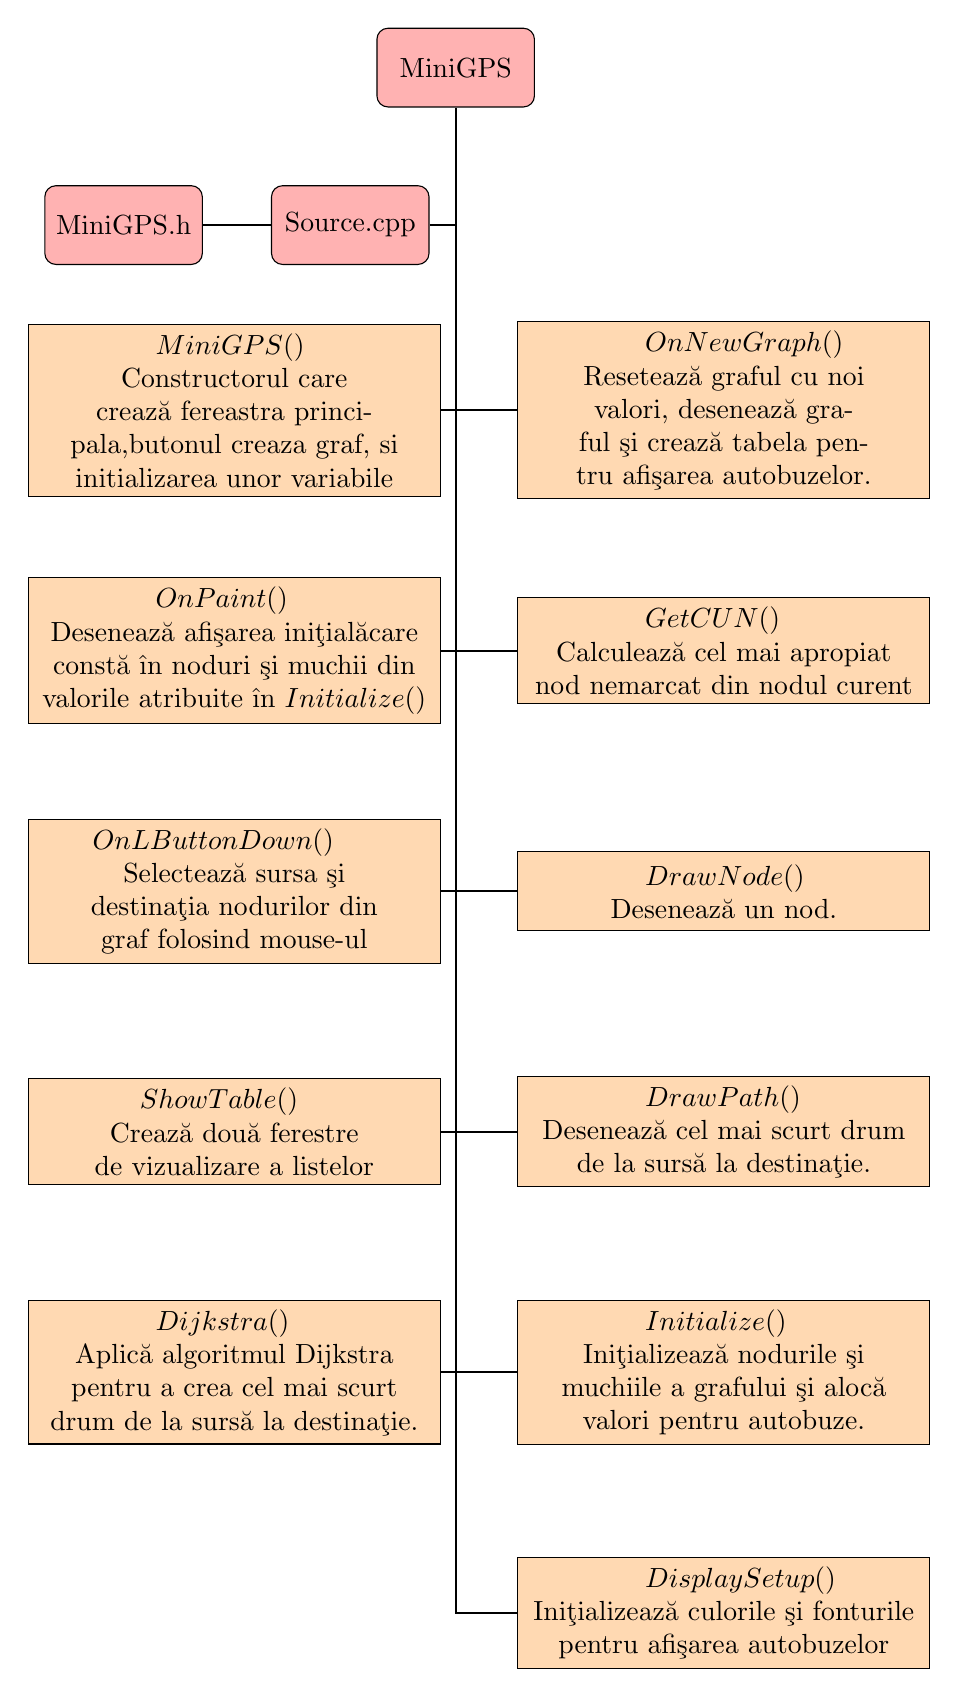
\begin{tikzpicture}[node distance=2cm]
\node (start) [startstop,xshift=-10em] {MiniGPS};
\node (MiniGPSS)   [startstop, below of=start,xshift=-12em] {MiniGPS.h};
\node (Source)  [startstop, right of=MiniGPSS,xshift=2.5em] {Source.cpp};
\node (MiniGPS)  [process, below of=MiniGPSS,yshift=-1em,xshift=4em] {\hspace{1.5cm}$MiniGPS()$ \newline Constructorul care creaz\u a fereastra principala,butonul creaza graf, si initializarea unor variabile};
\node (OnPaint)  [process, below of=MiniGPS,yshift=-3em] {\hspace{1.5cm}$OnPaint()$ \newline Deseneaz\u a afi\c sarea ini\c tial\u acare const\u a \^ in noduri \c si muchii din valorile atribuite \^ in $Initialize()$};
\node (OnLButtonDown)  [process, below of=OnPaint,yshift=-3em] {\hspace{0.7cm}$OnLButtonDown()$ \newline Selecteaz\u a sursa \c si destina\c tia nodurilor din graf folosind mouse-ul};
\node (ShowTable)  [process, below of=OnLButtonDown,yshift=-3em] {\hspace{1.3cm}$ShowTable()$ \newline Creaz\u a dou\u a ferestre de vizualizare a listelor};
\node (Dijkstra)  [process, below of=ShowTable,yshift=-3em] {\hspace{1.5cm}$Dijkstra()$ \newline Aplic\u a algoritmul Dijkstra pentru a crea cel mai scurt drum de la surs\u a la destina\c tie.};
\node (OnNewGraph)  [process, right of=MiniGPS,xshift=12em] {\hspace{1.5cm}$OnNewGraph()$ \newline Reseteaz\u a graful cu noi valori, deseneaz\u a graful \c si creaz\u a tabela pentru afi\c sarea autobuzelor.};
\node (GetCUN)  [process, right of=OnPaint,xshift=12em] {\hspace{1.5cm}$GetCUN()$ \newline Calculeaz\u a cel mai apropiat nod nemarcat din nodul curent};
\node (DrawNode)  [process, right of=OnLButtonDown,xshift=12em] {\hspace{1.5cm}$DrawNode()$ \newline Deseneaz\u a un nod.};
\node (DrawPath)  [process, right of=ShowTable,xshift=12em] {\hspace{1.5cm}$DrawPath()$ \newline Deseneaz\u a cel mai scurt drum de la surs\u a la destina\c tie.};
\node (Initialize)  [process, right of=Dijkstra,xshift=12em] {\hspace{1.5cm}$Initialize()$ \newline Ini\c tializeaz\u a nodurile \c si muchiile a grafului \c si aloc\u a valori pentru autobuze. };
\node (DisplaySetup)  [process, below of=Initialize,yshift=-3em] {\hspace{1.5cm}$DisplaySetup()$ \newline Ini\c tializeaz\u a culorile \c si fonturile pentru afi\c sarea autobuzelor};
\draw[arrow](MiniGPS)--(OnNewGraph);
\draw[arrow](OnPaint)--(GetCUN);
\draw[arrow](OnLButtonDown)--(DrawNode);
\draw[arrow](ShowTable)--(DrawPath);
\draw[arrow](Dijkstra)--(Initialize);
\draw[arrow](MiniGPSS)--(Source);
\draw[arrow](start)|-(DisplaySetup);
\draw[arrow](Source)-|(start);
\end{tikzpicture}
\newline

     Aceasta este schema pentru aplica\c tia MiniGPS. Sistemul mini-GPS pornc ste de la constructorul \textit{MiniGps()}, care creeaz\u a o fereastr\u a \c si butonul \textit{Graf nou}. Aceast\u a func\c tie apeleaz\u a deasemenea func\c tiile \textit{DisplaySetup()} \c si \textit{OnNewGraph} care stabile\c ste variabilele de afi\c sare comune \c si creeaz\u a graful. \textit{OnNewGraph()} apeleaz\u a \textit{Initialize} care creeaz\u a graful prin alocarea coordonatelor aleatorii la noduri \c si costul aleatorii la muchiile grafului. Graful initial este afi\c sat \c si updatat prin \textit{OnPaint()}.
     
     Evenimentul \textit{ON\_WM\_LBUTTONDOWN()} detecteaz\u a clik-ul din st\^ anga mous-ului a c\u a rui pozi\c tie se afl\u a \^ in Windows returnat de obiectul \textit{CPoint pt}. Valoarea obiectului este verificat\u a cu \textit{v[i].rct} folosind \textit{PtInRect()}. Nodul surs\u a este identificat prin \textit{bFlag=1} iar destina\c tia prin \textit{bFlag=2}.
     
     \textit{Dijkstra()} calculeaz\u a cel mai scurt drum folosing algoritmul lui Dijkstra. Func\c tia este apelat\u a atunci c\^ and nodul secund a fost selectat \^ in timp ce autobuzul de la surs\u a la nodul destina\c tie este desenat folosind \textit{DrawPath()}. Odata ce primul autobuz a fost finalizat, informa\c tiile sale sunt actualizate \c si afi\c sate \^ in fereastra de vizualizare. Deasemenea , muchiile de la primul autobuz sunt \c sterse din graful original. \c Stergerea muchiilor este \^ indeplinit\u a de \textit{Initialize()} \^ inlocuind valoarea muchiei cu 99.
     
     Cel de-al doilea autobuz este o repetare a primului autobuz prin referire la graful redus G'. Prin urmare, calculul pentru noul drum dintre cele dou\u a noduri, va lua \^ in considerare faptul c\u a primul drum are noduri neadiacente dealungul parcurgerii. Programul calculeaz\u a noul drum care \^ in mod cert avit\u a primul drum. Similar, se aplic\u a aceea\c si metod\u a \c si pentru drumul cu num\u a rul 3.
\end{document}
